\section{Methodology}

Physics-Informed Neural Networks (PINNs) represent a recent advancement in machine learning for solving inverse problems constrained by partial differential equations (PDEs) \cite{raissi2019,karniadakis2021physics}. By integrating the underlying physics into the neural network's loss function, PINNs can accurately reconstruct complex dynamical systems even when available data is sparse. Unlike conventional neural networks that rely heavily on large volumes of labeled data, PINNs leverage domain knowledge in the form of PDEs, enabling faster and more physically consistent learning \cite{cuomo2022scientific,mao2020physics}.

The anisotropic Eikonal equation provides a mathematical model for simulating electrical activation in cardiac tissue, explicitly accounting for the direction-dependent effects of fiber orientation on wavefront propagation \cite{ColliFranzone1990, Grandits2021Springer}. We integrate this equation into the proposed PINN framework as the governing physical constraint embedded within the learning process.

The anisotropic Eikonal equation governs the activation time $\phi(\mathbf{x})$ at each spatial location $\mathbf{x}$ as follows \cite{Grandits2021Springer}:
\begin{equation}
    \sqrt{ \mathbf{D}(\mathbf{x}) \nabla \phi(\mathbf{x}) \cdot \nabla  \phi(\mathbf{x})} = 1
\end{equation}
where $\mathbf{D}(\mathbf{x})$ is the local conduction velocity tensor that encodes directional variations in wavefront speed due to underlying myocardial fiber architecture. Unlike isotropic models that assume uniform conduction in all directions, this anisotropic formulation enables the model to capture direction-dependent conduction patterns—crucial for physiologically accurate activation maps.

To infer activation times and conduction velocity tensors from sparse intracardiac catheter data, we utilize a dual-network PINN architecture. One network approximates the activation time $\phi(\mathbf{x})$, while the other approximates the conduction velocity tensor $\mathbf{D}(\mathbf{x})$, as shown in Fig. \ref{fig:NNArch}, ensuring that the solution remains consistent with the anisotropic Eikonal equation.

\begin{figure}
    \centering
    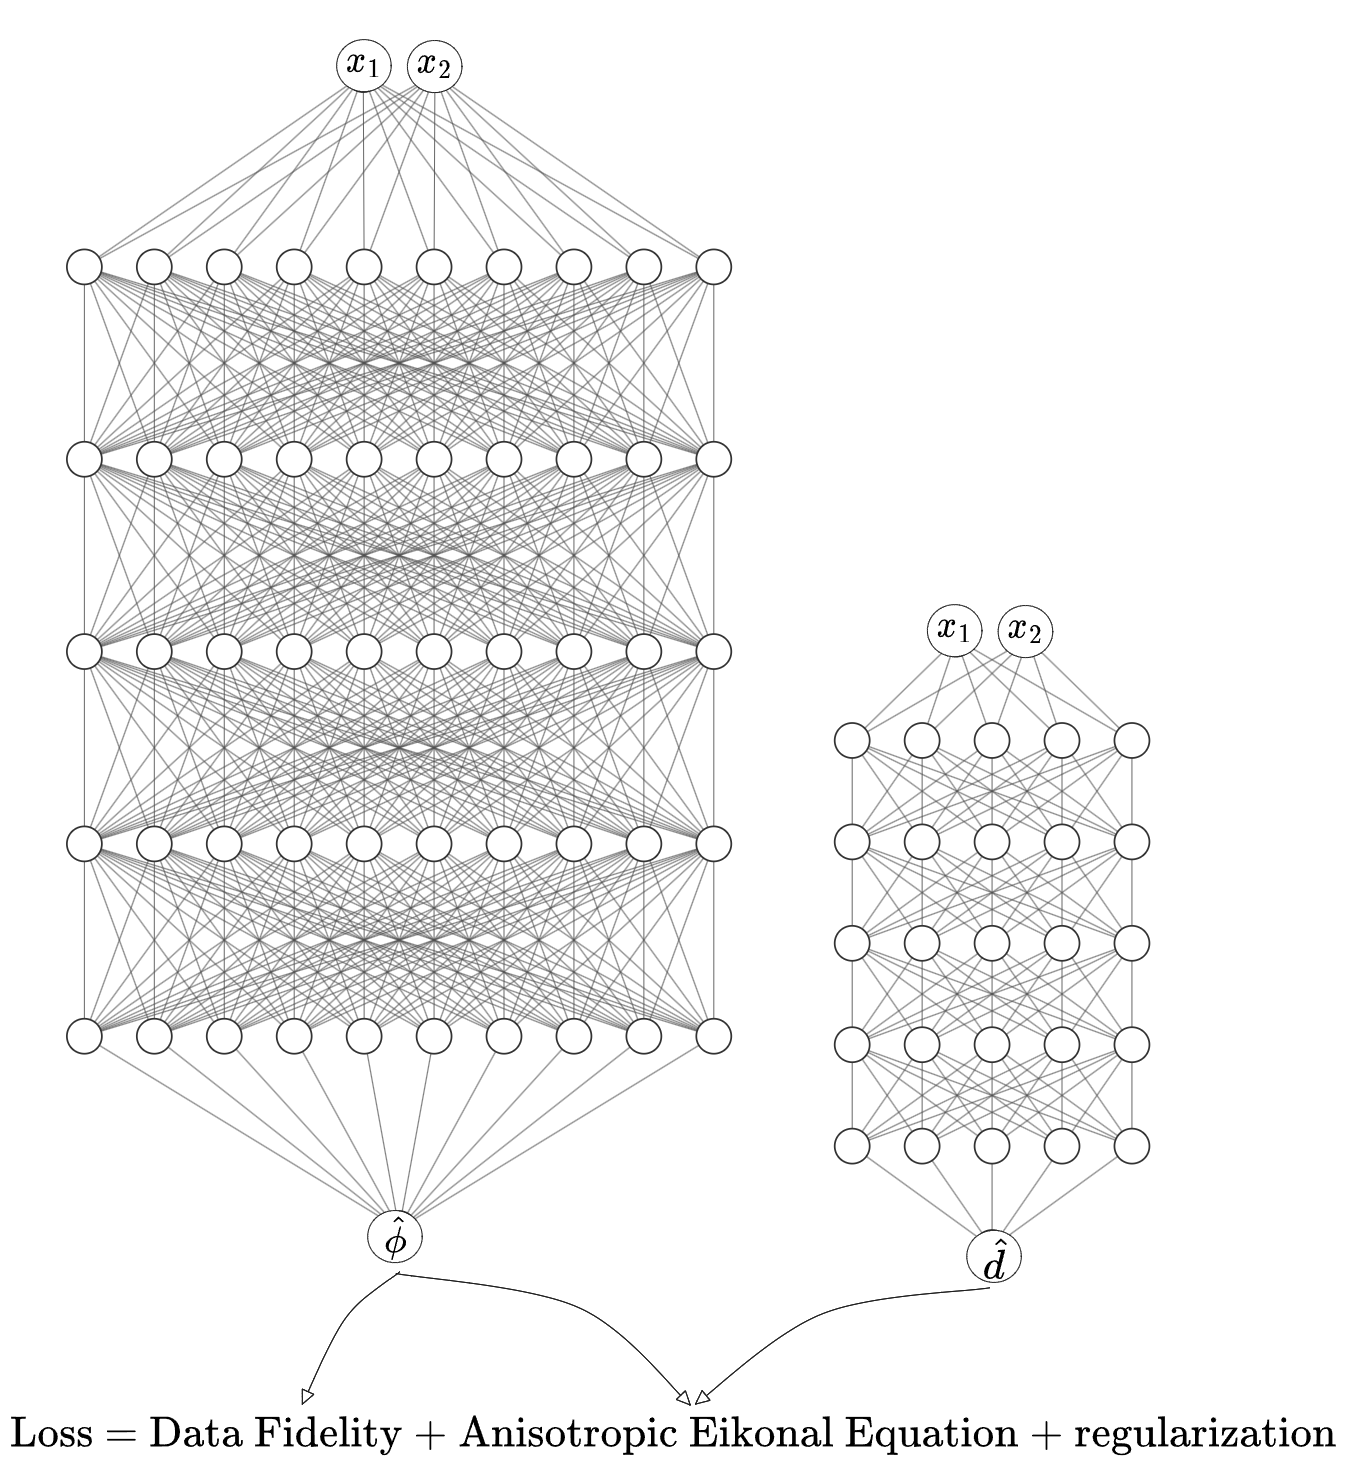
\includegraphics[width=1\linewidth]{figures/NeuralNet.png}
    \caption{
    Schematic representation of the physics-informed neural network architecture used in this study. The framework consists of two neural networks: one network estimates the conduction velocity tensor field (right neural network), while the other predicts the activation time across the spatial domain (left neural network).
    }
    \label{fig:NNArch}
\end{figure}

\subsection{Neural Networks Architecture}


\textbf{Activation Time Network} ($\text{NN}_\phi$): The first neural network, composed of five hidden layers with ten neurons per layer and parameterized by $\theta_\phi$, approximates a scalar activation time given 2D spatial input coordinates $\mathbf{x}$.
\begin{equation}
\hat{\phi}(\mathbf{x}) := \text{NN}_\phi(\mathbf{x}; \theta_\phi)
\end{equation}

\textbf{Velocity Tensor Network} ($\text{NN}_D$): The second neural network, parameterized by $\theta_D$, consists of five hidden layers with five neurons each. It maps the spatial coordinates $\mathbf{x}$ to a set of intermediate parameters that define a symmetric and positive-definite conduction velocity tensor. We denote this parameter set as $\mathbf{d}(\mathbf{x})$, where

\begin{equation}
    \mathbf{d}(\mathbf{x}) = [e_1(\mathbf{x}), e_2(\mathbf{x}), a(\mathbf{x})],
\end{equation}

with $e_1$ and $e_2$ representing the squared conduction speeds along the longitudinal and transverse fiber directions, respectively, and $a$ denoting the local fiber orientation angle. The network output is defined as

\begin{equation}
    \hat{\mathbf{d}}(\mathbf{x}) := \text{NN}_D(\mathbf{x}; \theta_D).
\end{equation}

To reconstruct the conduction velocity tensor $\mathbf{D}(\mathbf{x})$, we rotate the diagonal tensor composed of $e_1$ and $e_2$ using the fiber orientation angle $a(\mathbf{x})$ \cite{Arsigny2007}:

\begin{equation}
\mathbf{D}(\mathbf{x}) = R(a(\mathbf{x}))^\top 
\begin{bmatrix}
e_1(\mathbf{x}) & 0 \\
0 & e_2(\mathbf{x})
\end{bmatrix}
R(a(\mathbf{x}))
\end{equation}

where the 2D rotation matrix $R(a)$ is given by:
\begin{equation}
R(a) = 
\begin{bmatrix}
\cos a & -\sin a \\
\sin a & \cos a
\end{bmatrix}
\end{equation}

\subsection{Loss Function and Optimization}

The training objective is defined as a composite loss:
\begin{equation}
\mathcal{L}(\theta_\phi, \theta_D) = \mathcal{L}_{\text{data}} + \alpha_{\text{eiko}} \mathcal{L}_{\text{eiko}} + \alpha_{\text{reg}} \mathcal{L}_{\text{reg}}
\end{equation}

\textbf{Data Loss} ($\mathcal{L}_{\text{data}}$): Penalizes deviation from observed activation times at known $N_d$ data points:
\begin{equation}
\mathcal{L}_{\text{data}} = \frac{1}{N_d} \sum_{i=1}^{N_d} \left(\hat{\phi}(\mathbf{x}_i) - \phi(\mathbf{x}_i)\right)^2
\end{equation}

\textbf{Eikonal Residual Loss} ($\mathcal{L}_{\text{eiko}}$): Enforces satisfaction of the anisotropic Eikonal equation at $N_c$ collocation points:
\begin{equation}
    \mathcal{L}_{\text{eiko}} = \frac{1}{N_c} \sum_{j=1}^{N_c} \left(\sqrt{ \mathbf{\hat D}(\mathbf{x}_j) \nabla \hat{\phi}(\mathbf{x}_j) \cdot \nabla \hat{\phi}(\mathbf{x}_j)} - 1\right)^2
\end{equation}


\textbf{Regularization Loss} ($\mathcal{L}_{\text{reg}}$): To encourage spatial regularity, we incorporate Huber total variation $\left(\text{TV}_{\text{Huber}}\right)$ as a penalization term, as it has been demonstrated to favor piecewise constant structures in the estimated fields \cite{Chambolle_Pock_2016}.
\begin{equation}
    \mathcal{L}_{\text{reg}} = \sum_{k \in \{e_1, e_2, a\}} \text{TV}_{\text{Huber}}(k(\mathbf{x}))
\end{equation}


This formulation enables physically consistent inference of activation patterns while explicitly modeling the impact of fiber orientation, a critical determinant of wavefront propagation in realistic cardiac tissue.

The proposed framework is implemented in TensorFlow \cite{abadi2016tensorflowlargescalemachinelearning}. The neural networks are trained by minimizing the total loss function using the ADAM optimizer \cite{kingma2017adammethodstochasticoptimization}, thereby learning the parameters $\theta_\phi$ and $\theta_D$.